\documentclass[hyperref={pdfpagelabels=false}]{beamer}
\let\Tiny=\tiny
\mode<presentation>{
\usetheme{AnnArbor}
\usecolortheme{beaver}
\usefonttheme{serif}
}
\usepackage{default}
%\usepackage{ucs}
\usepackage[utf8]{inputenc}
\usepackage{gb4e}
\usepackage[T1]{fontenc}
\usepackage{ tipa }
\usepackage{qtree}
\usepackage{synttree}
%\usepackage{color}
\usepackage{tree-dvips}
\usepackage[absolute,overlay]{textpos}
%\usepackage{covington-beamer}
\usepackage{lmodern}
\usepackage{hyperref}
\usepackage{natbib}
\usepackage{graphicx}
\usepackage{eso-pic}
\usepackage{booktabs}
\usepackage{tikz}
%\usepackage{memoir}
%\usepackage{relsize}
%\newcommand{\subscript}[1]{\raisebox{-0.25em}{\smaller #1}}
%\logo{\includegraphics[height=1cm]{nclcbelogomono.eps}}
\setbeamertemplate{footline}[frame number] 
%gets rid of navigation symbols
\setbeamertemplate{navigation symbols}{}

\title{An information theoretic approach to language change}
\author{Joel C. Wallenberg\\\texttt{joel.wallenberg@ncl.ac.uk}}
\institute{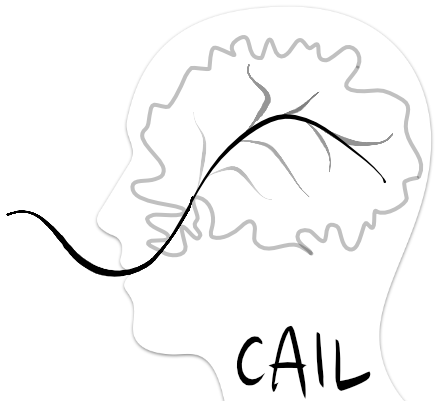
\includegraphics[scale = 0.2]{caillogo.png}}
%\date[]{14th May, 2019}

\begin{document}

\begin{frame}[plain]
\titlepage
\end{frame}




\begin{frame}{``Constraints on the Adaptiveness of Information in Language'' (CAIL)} 
	
	\begin{itemize}
		\item \small{\url{https://cail-project.github.io/}}
		\item Collaboration with Christine Cuskley and Rachael Bailes
		\item ESRC Secondary Data Analysis Initiative (SDAI), grant \#ES/T005955/1\\

	\end{itemize}


	\begin{center}
		\includegraphics[scale=0.2]{wallenbergetalheader.png}
	\end{center}
\rightline{\textsl{\citet{wallenbergetal2021}}}


\end{frame}

\begin{frame}{A Mystery in Language Change} 
	
	\begin{itemize}
		\item A \textbf{Constant Rate Effect} \small{(first described in \citealt{kroch1989})}: when a change in some linguistic variable is in progress, some linguistic contexts favour one variant over another \textbf{without changing the change} (i.e. stopping, slowing, accelerating, etc.).\pause
		\item Using information theory, we can not only explain a CRE, but predict the existence of one.\pause
		\item This CRE shows speakers unconsciously solving a complex planning problem to achieve \textbf{information uniformity}.
	\end{itemize}
	
\end{frame}

\begin{frame}{OV-to-VO in English and Icelandic} 
	
	
	\textbf{Middle English:}
	\begin{exe}	
		\ex \label{julia}  \gll Mi feader \& Mi moder for-þi þt ich nule þe forsaken; habbe forsake me.\\
		My father and my mother because that I not+would you forsake have forsaken me\\
		\quad ``Because I would not forsake you, my father and mother have forsaken me''\\\vspace{2mm}
		\small{(\textsl{St. Juliana}, northern Herefordshire/southern Shropshire, date: c1225; ID CMJULIA-M1,106.172 from the \textsl{Penn Parsed Corpus of Middle English 2} \citep{ppcme24})}
	\end{exe}
	
\end{frame}

\begin{frame}{OV-to-VO in English and Icelandic} 
	
	\textbf{Historical Icelandic:}%This is not a list
	\begin{exe}\ex \label{ex:ntov}\begin{xlist}
			\ex {\gll \ldots og sannleikurinn mun yður frelsa \\
				\ldots and {the truth} will you free \\
				\quad ``\ldots and the truth will set you free.''  }\\\vspace{2mm}
			\small{(\textit{\small{Oddur Gottskálksson's New Testament}}, date: 1540; ID 1540.NTJOHN.REL-BIB, 204.662 from \textsl{Icelandic Parsed Historical Corpus} \citep{icepahc09})}\\\vspace{5mm}
			%1540.NTJOHN.REL-BIB,204.662
			\ex {\gll \ldots en eg skal sjá yður aftur. \\
				but I shall see you-\sc{pl} again\\
				\quad ``\ldots but I shall see you again'' \\\vspace{2mm}
				\small{(\textit{Oddur Gottskálksson's New Testament}, date: 1540; ID 1540.NTJOHN.REL-BIB, 223.1305 from IcePaHC)}
				% 1540.NTJOHN.REL-BIB,223.1305   
			}
		\end{xlist}
	\end{exe}
	
	
	
\end{frame}

\begin{frame}{OV-to-VO in English and Icelandic} 
	
	
	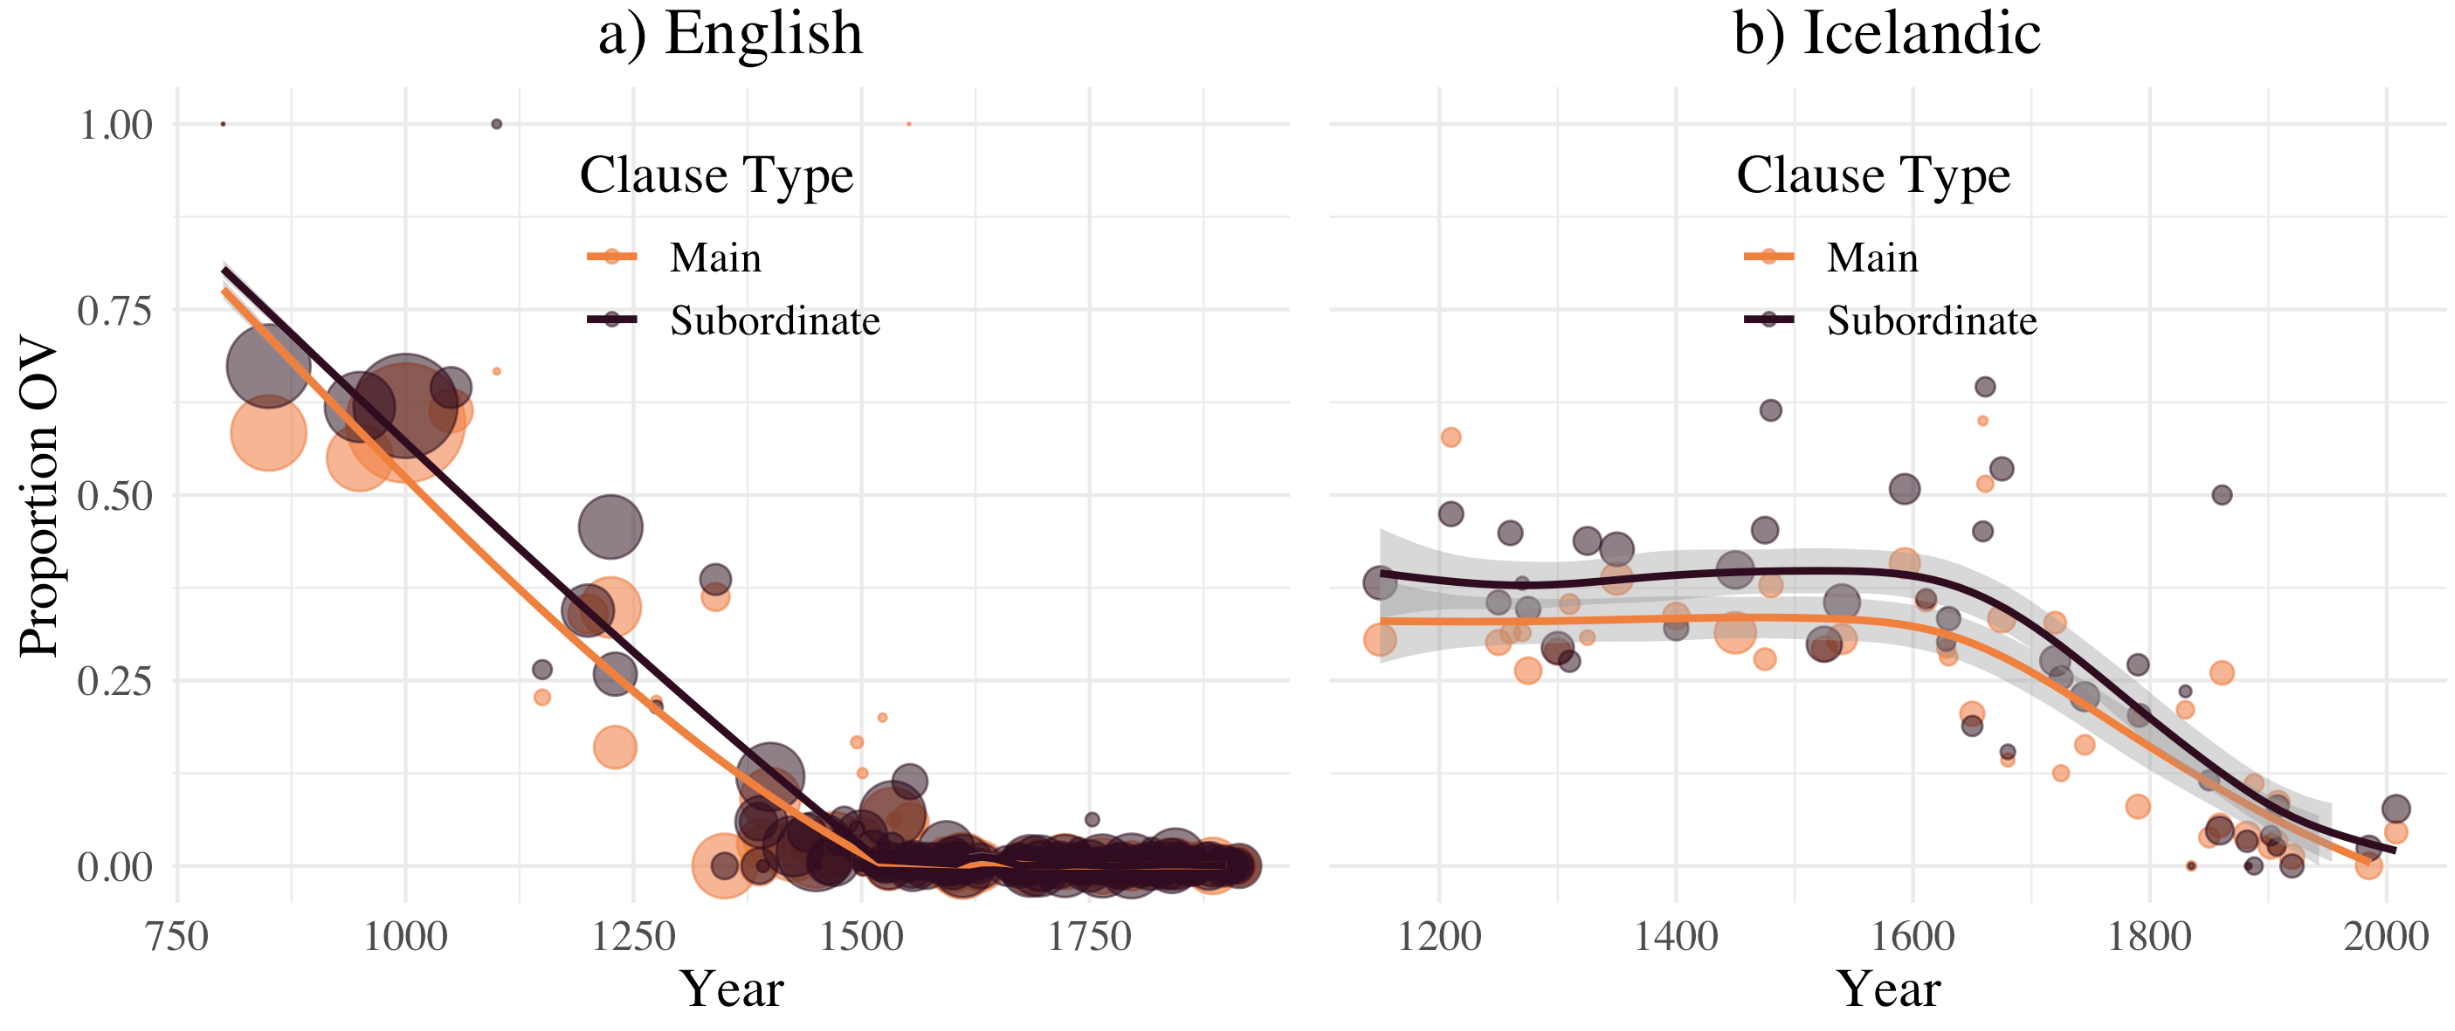
\includegraphics[width=1.04\textwidth]{FullClauseFig.png}
	\begin{itemize}
		\item Note the Constant Rate Effect (CRE), shown for English by \citet{pintzuktaylor2006}.
	\end{itemize}	
\end{frame}




\begin{frame}
	\frametitle{Outline}
	\tableofcontents
\end{frame}


\section{Crash Course in Information Theory}

\begin{frame}{Crash course: Information theory and language} 

\begin{center}

	\includegraphics[scale=0.55]{../shannonSchematic.png} 


\end{center}\pause
\begin{itemize}
	\item \textbf{Key Insight:} The amount of information a sender can theoretically communicate about an event is the uncertainty (``entropy'') the receiver has about the event beforehand, which may be reduced by a signal \citep{hartley1928, shannon1948}.
\end{itemize}


\end{frame}

\begin{frame}{Crash course: Information theory and language} 
	\begin{itemize}
		\item The more unexpected for the receiver, the more information.\pause
	\end{itemize}
	\begin{center}
			\includegraphics[scale=0.4]{bbcweather.jpg} 
	\end{center}
\end{frame}


\begin{frame}{Crash course: Information theory and language} 
	\begin{itemize}
		\item \citet{shannon1948}'s formula for information in an event with \textsl{n} discrete outcomes with probabilities p_1...p_n:
	\end{itemize}
	\begin{center}
		$$\sum_{1}^{n} p_i log_2 \frac{1}{p_i}$$
	\end{center}
	\begin{itemize}
		\item The $log_2 \frac{1}{p_i}$ part is the \textsl{information content} of an outcome.
		\item Lower probability signals provide more information when received, though they show up less often.
		\item The unit of information is a \textbf{``bit''}!
	\end{itemize}
	
\end{frame}


\begin{frame}{``Information Uniformity'' in Sentences} 
\begin{itemize}
	\item Suppose morphemes, words, phrases are signals to the overall interpretation/function of an utterance.\\\vspace{5mm}
	\begin{itemize} \item[] \textbf{low probability $\rightarrow$ high information content}\pause\\\vspace{5mm}  \end{itemize}
	\item Speakers tend to spread information across utterances as uniformly as possible, perhaps to mitigate effects of ``noise'':\\ \begin{itemize}
		\item[] \footnotesize{(\citealt{fenkfenk1980,aylettturk2004,levyjaeger2007}; Cuskley, Bailes \& Wallenberg, \textsl{Forthcoming})}\nocite{cuskleyWallenberg2021}
	\end{itemize}
\end{itemize}



\end{frame}



\begin{frame}{``Information Uniformity'' in Sentences} 

\begin{center}
\includegraphics[scale=0.585]{../sentence1info.png} 
\end{center}

\end{frame}

\begin{frame}{``Information Uniformity'' in Sentences} 

\begin{center}
	\includegraphics[scale=0.585]{../sentence2info.png} 
\end{center}

\end{frame}


\section{Study 1: OV-to-VO in English and Icelandic}


\begin{frame}{OV-to-VO and Information Theory} 
	
	\begin{center}
		
		 \textbf{OV: Sbj Aux Obj V}\\
		\textbf{VO: Sbj Aux V Obj}\\\vspace*{5mm}\pause
\begin{tabular}{c c}
	
	\textbf{Constituent Type} & \textbf{Average Information Content} \\ \hline
	Pronominal DP & low ($\approx$ 11.7 bits)\\
	Nominal DP & HIGH ( > 13.7 bits) \\
	Lexical  Verb & \textsc{mid} ($\approx$ 13.5 bits) \\
\end{tabular}\pause
\\\vspace*{5mm}
\textbf{Hypothesis_1:} VO is favoured when Sbj and Obj are the same type.\pause\\\vspace*{1mm} (low \textsc{mid} low , HIGH \textsc{mid} HIGH) \textbf{vs} (low low \textsc{mid}, HIGH HIGH \textsc{mid})  \\\vspace*{4mm}\pause
\textbf{Hypothesis_2:} OV is favoured when Sbj, Obj are \textbf{NOT} the same type.\pause\\\vspace{1mm} (low HIGH \textsc{mid} , HIGH low \textsc{mid}) \textbf{vs} (low \textsc{mid} HIGH, HIGH \textsc{mid} low)\\\vspace*{4mm}\pause
\textbf{Hypothesis_3:} These effects are orthogonal to the change (a CRE).
\end{center}
\end{frame}

\begin{frame}{OV-to-VO and Information Theory} 


\begin{exe}	
	\ex \gll sua sal ye yure sinnes les.\\
so shall {you (\textbf{\small{low}})} your {sins (\textbf{HIGH})} {lose \textbf{(\textsc{mid})}}\\
\quad ``In this way, you will let go of your sins.''\\
(\textsl{Rule of St. Benet}, Yorkshire, date: 1425)\\\vspace{5mm}


\end{exe}
\end{frame}


\begin{frame}
	
	\begin{center}
	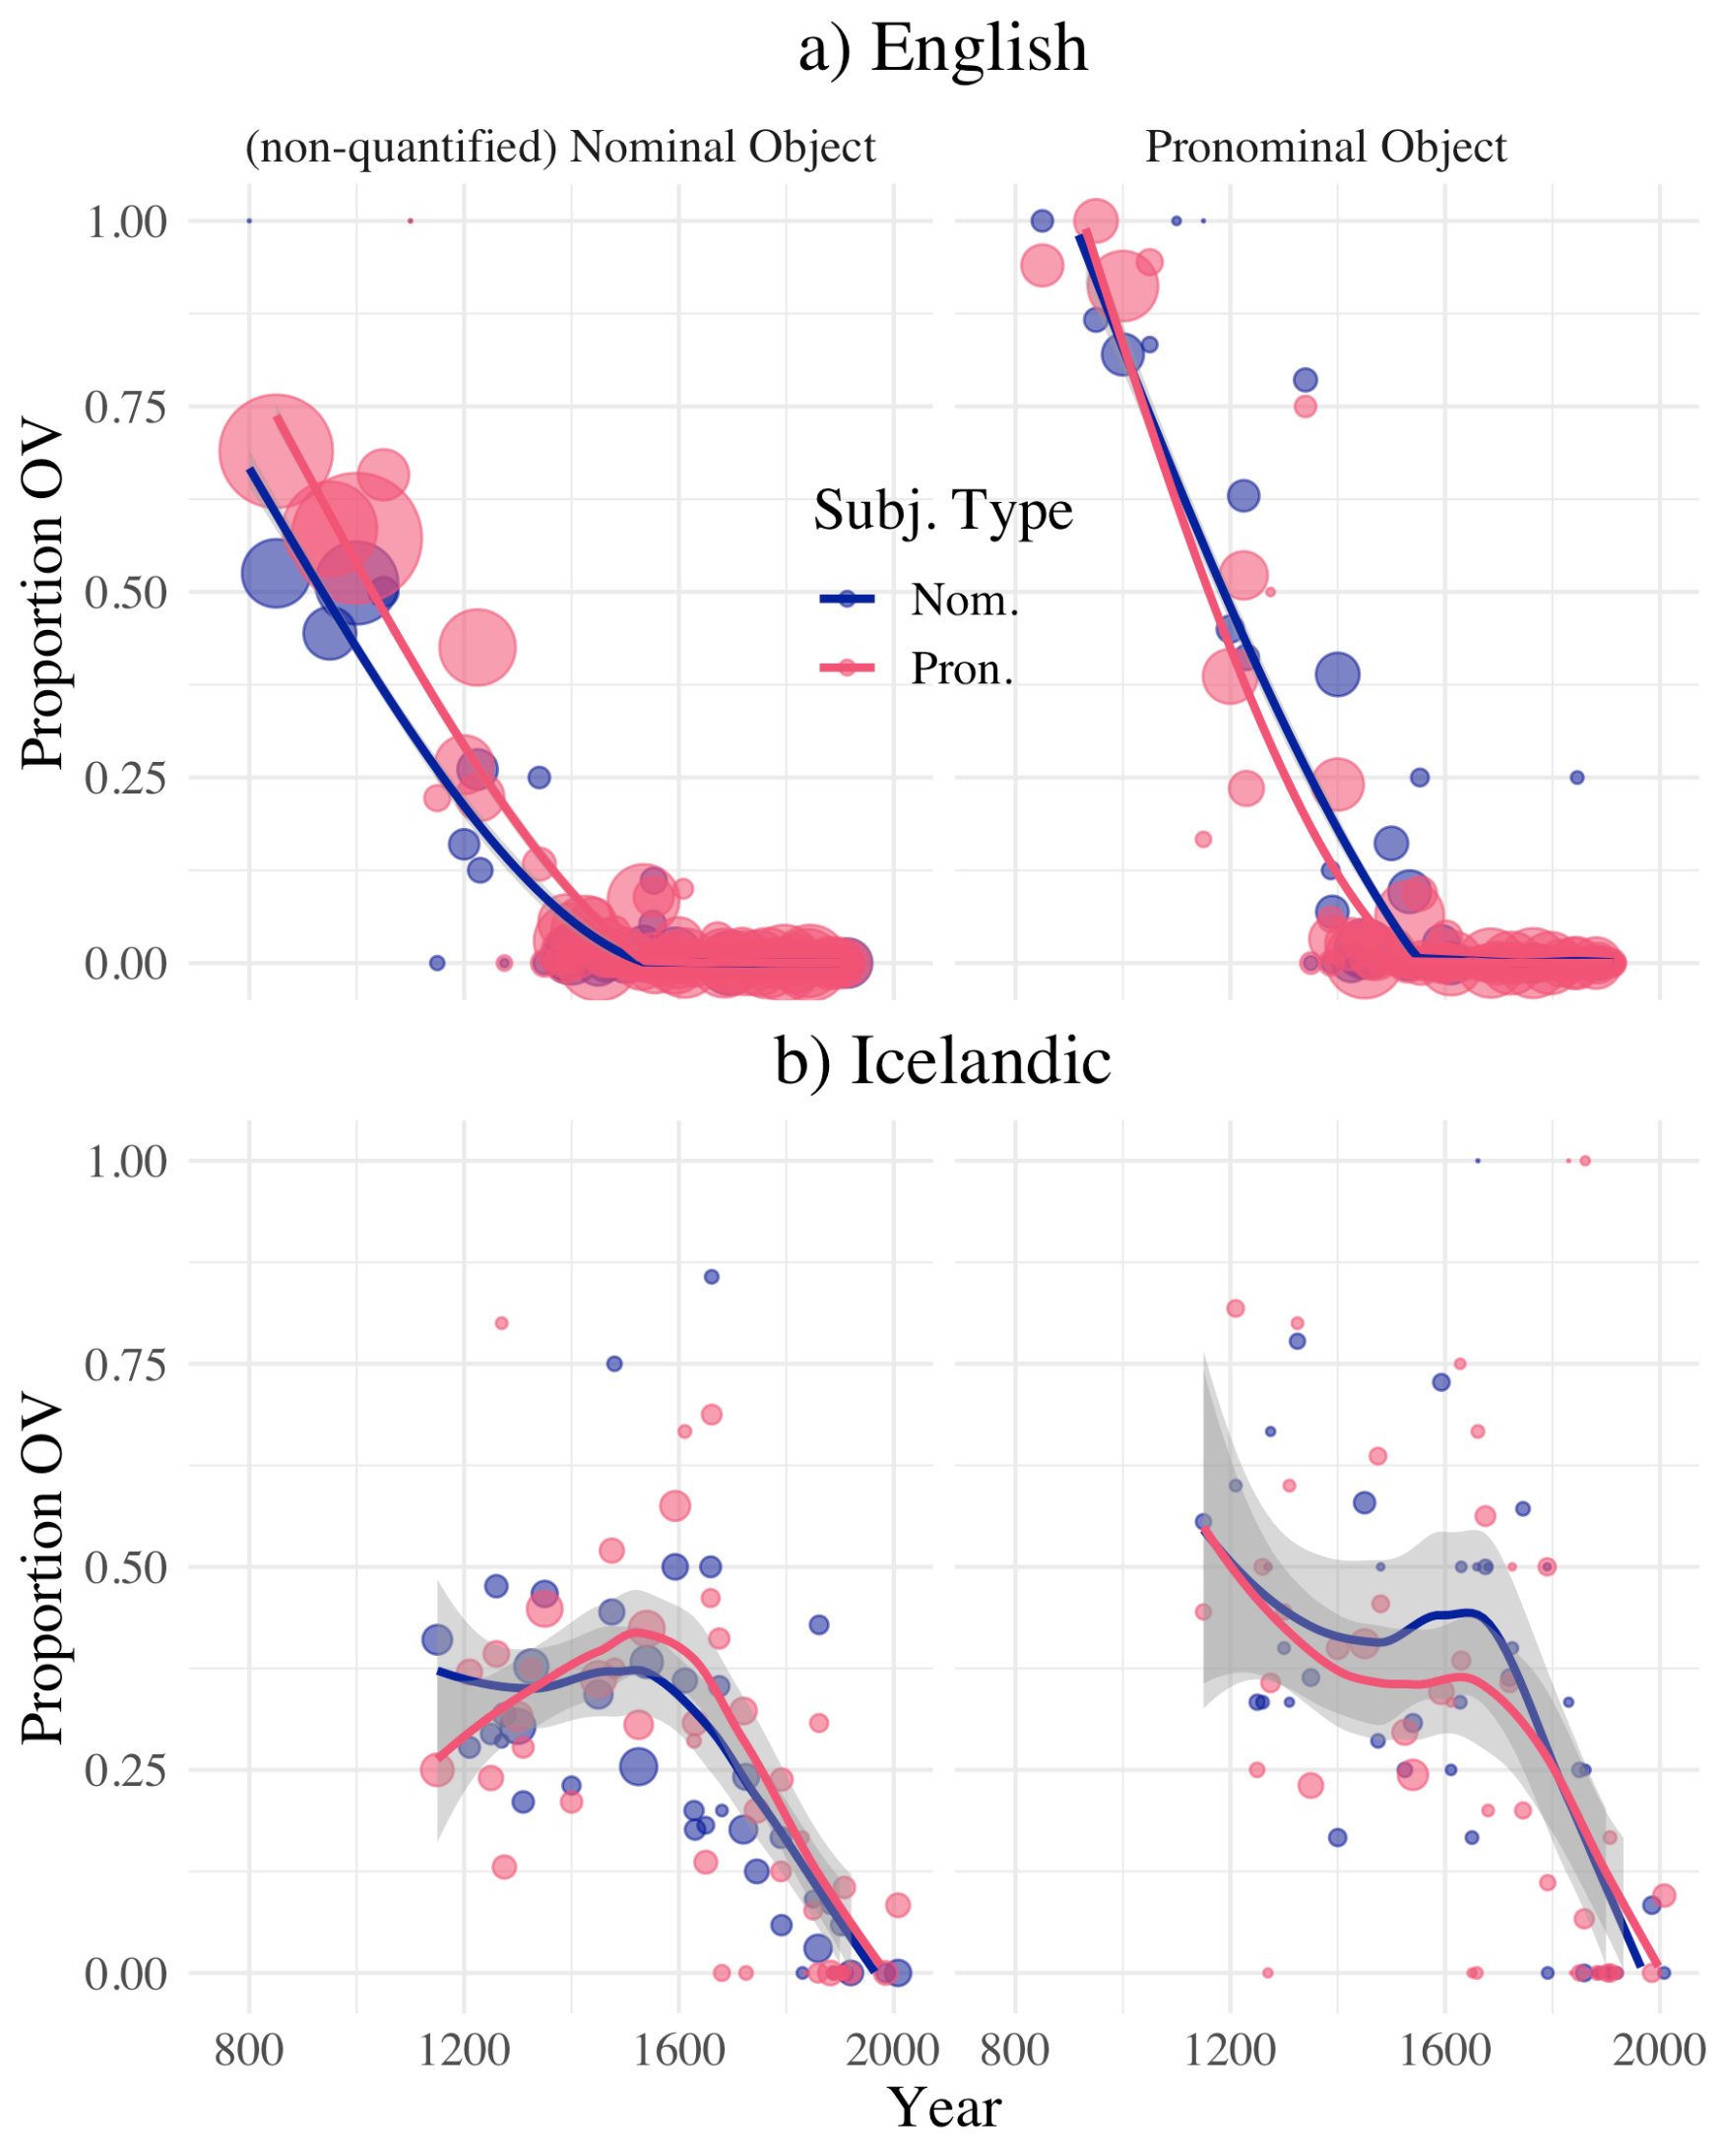
\includegraphics[scale = 0.5]{Fig3-4.png}
	\end{center}
\end{frame}



\section{Study 2: OV and VO variation in historical Icelandic}


\begin{frame}{More detail: OV and VO variation in historical Icelandic} 

\begin{itemize}
	\item ``DORM'': Deviation of the Rolling Mean
	\item A \textbf{summary statistic} for how informationally uniform a sentence is (Cuskley, Bailes \& Wallenberg, \textsl{Forthcoming}).\pause
\end{itemize}
	\begin{center}
		 \textbf{low DORM} $\rightarrow$ \textbf{more uniform}\\
		 \textbf{high DORM} $\rightarrow$ \textbf{more lopsided}
	\end{center}\pause
\begin{itemize}

	\item Based on strings of lemmas for Icelandic sentences, due to large number of morphological forms (and some spelling variation) in the Icelandic Parsed Historical Corpus \citep{icepahc09}.
\end{itemize}

\end{frame}


\begin{frame}{DORM and OV-to-VO in Icelandic} 
	
	\begin{center}

		\textbf{low DORM} $\rightarrow$ \textbf{more uniform}\\
		\textbf{high DORM} $\rightarrow$ \textbf{more lopsided}\\\vspace{4mm}
		\textbf{Hypothesis_1:} When Sbj and Obj are same type, OV results in higher DORM.\\\pause
		\textbf{Hypothesis_2:} When Sbj and Obj are different types, OV results in lower DORM.\\\pause
		\textbf{Hypothesis_3:} These effects are orthogonal to the change (a CRE).\\
	\end{center}
	
\end{frame}






\begin{frame}%{OV, OV, and Information Uniformity in Icelandic} 
	
	
	\begin{center}
	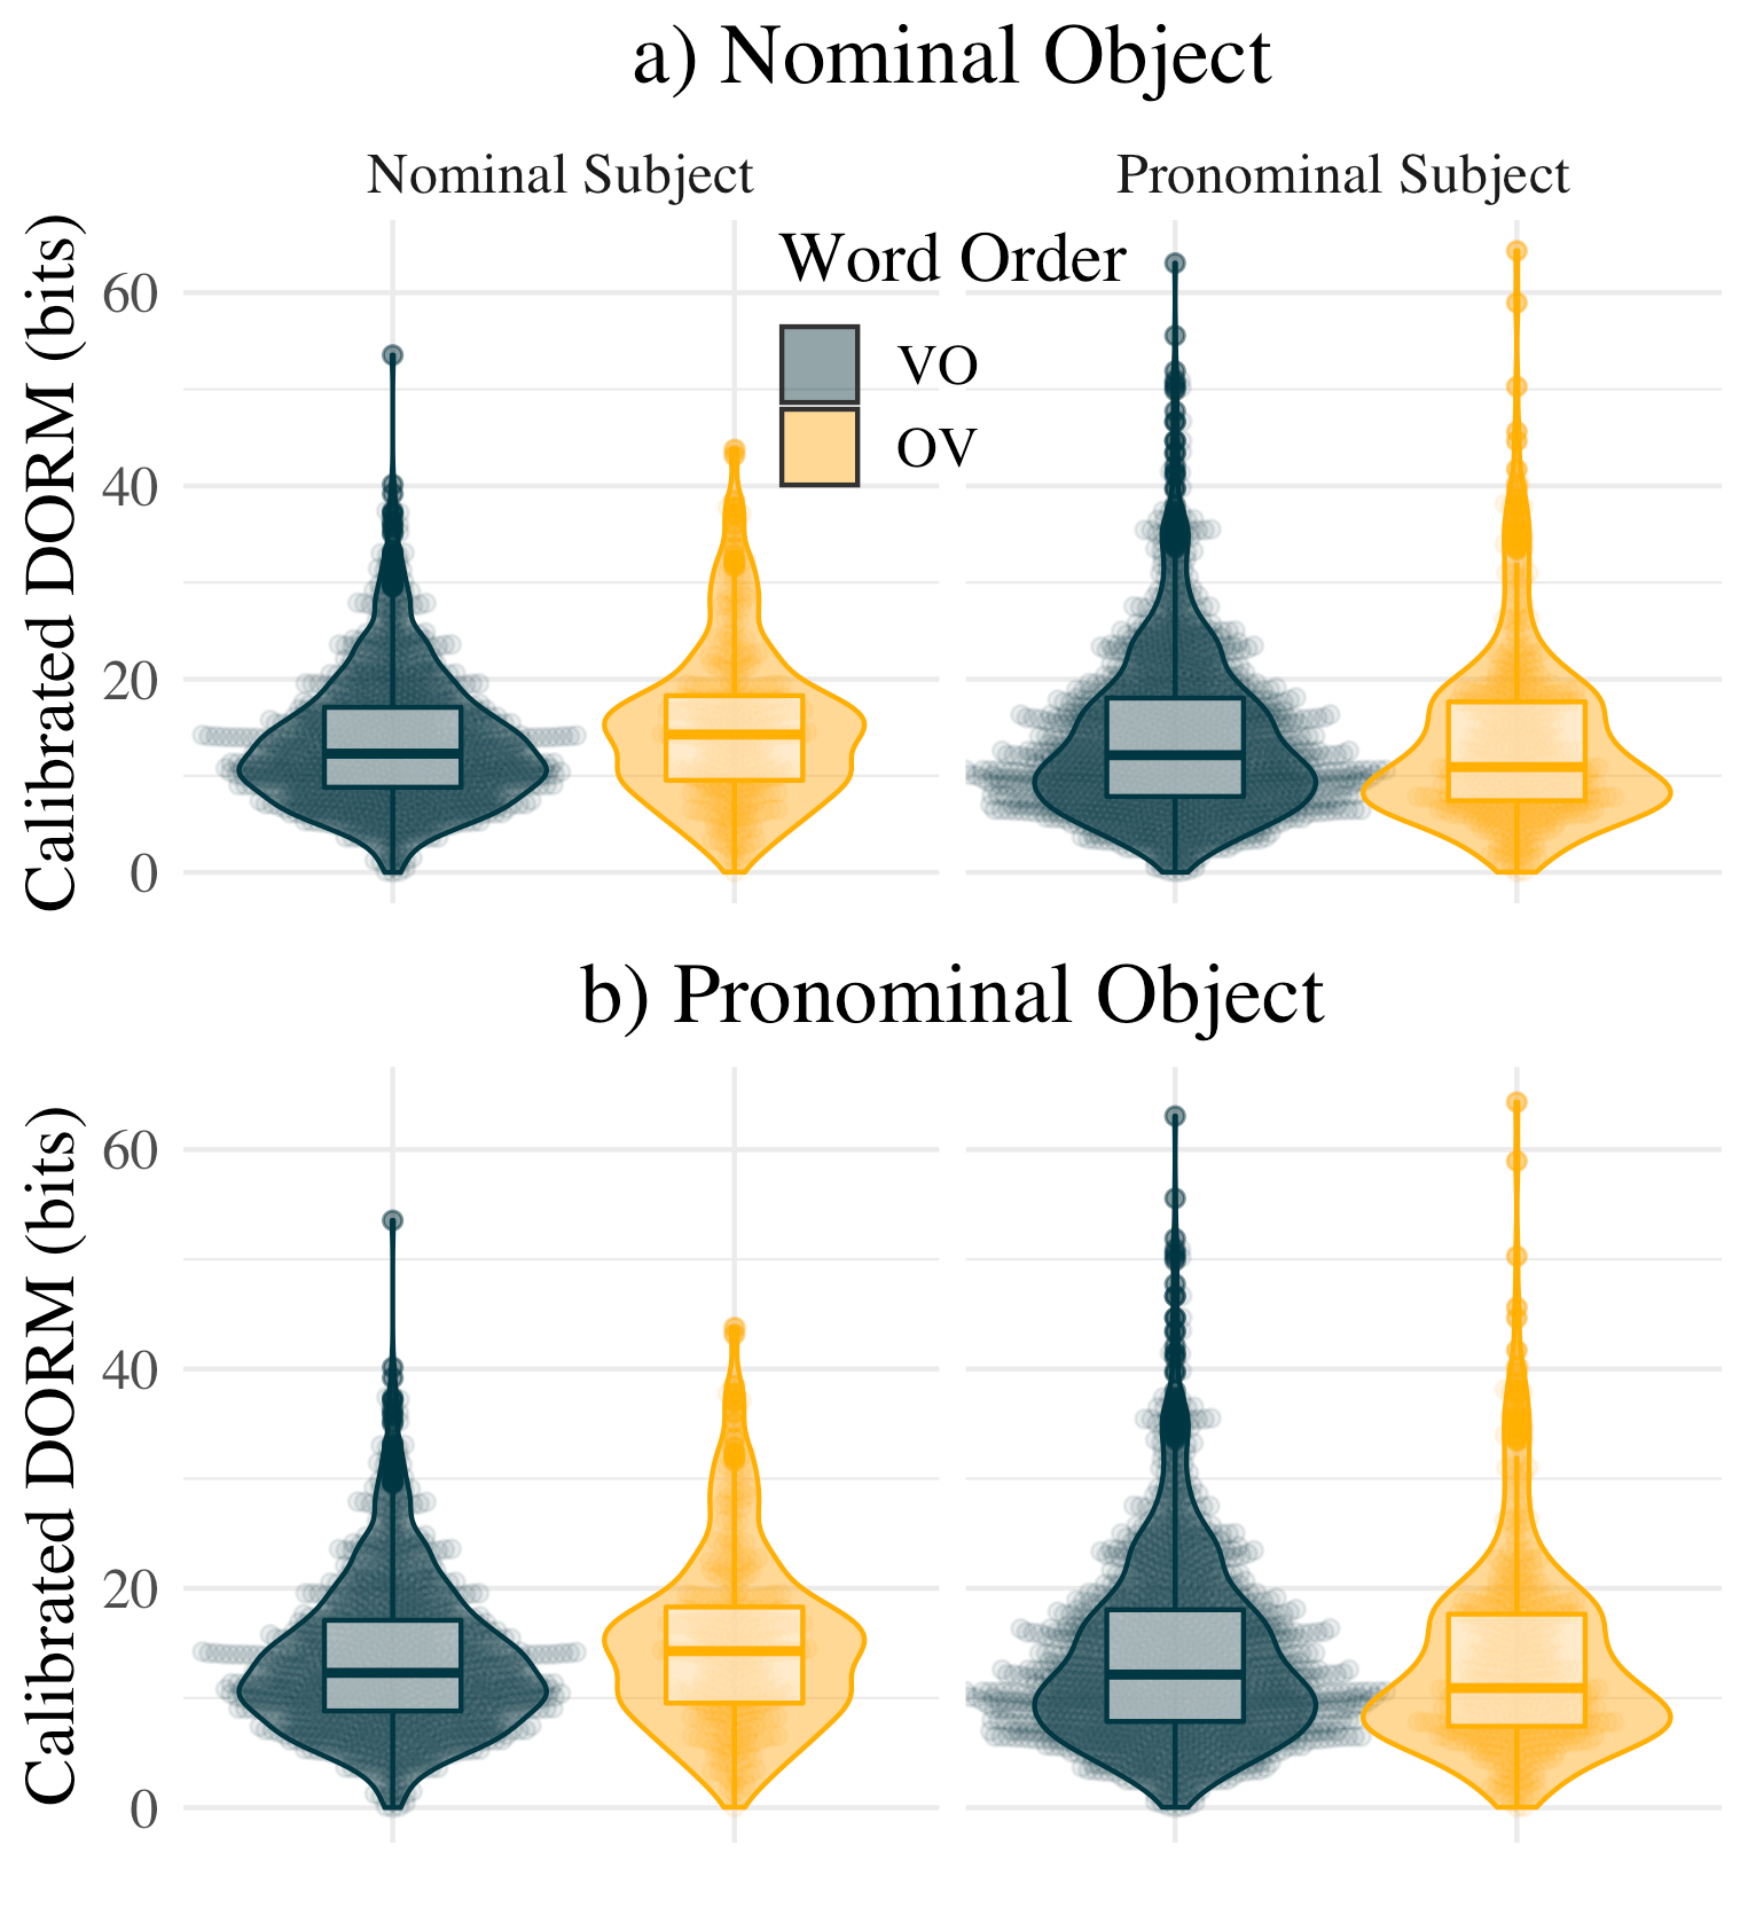
\includegraphics[scale = 0.57]{NewFigType3.png}
\end{center}
	
\end{frame}

\begin{frame}{What Doesn't Change, Doesn't Change} 
	
	
%	\begin{center}
		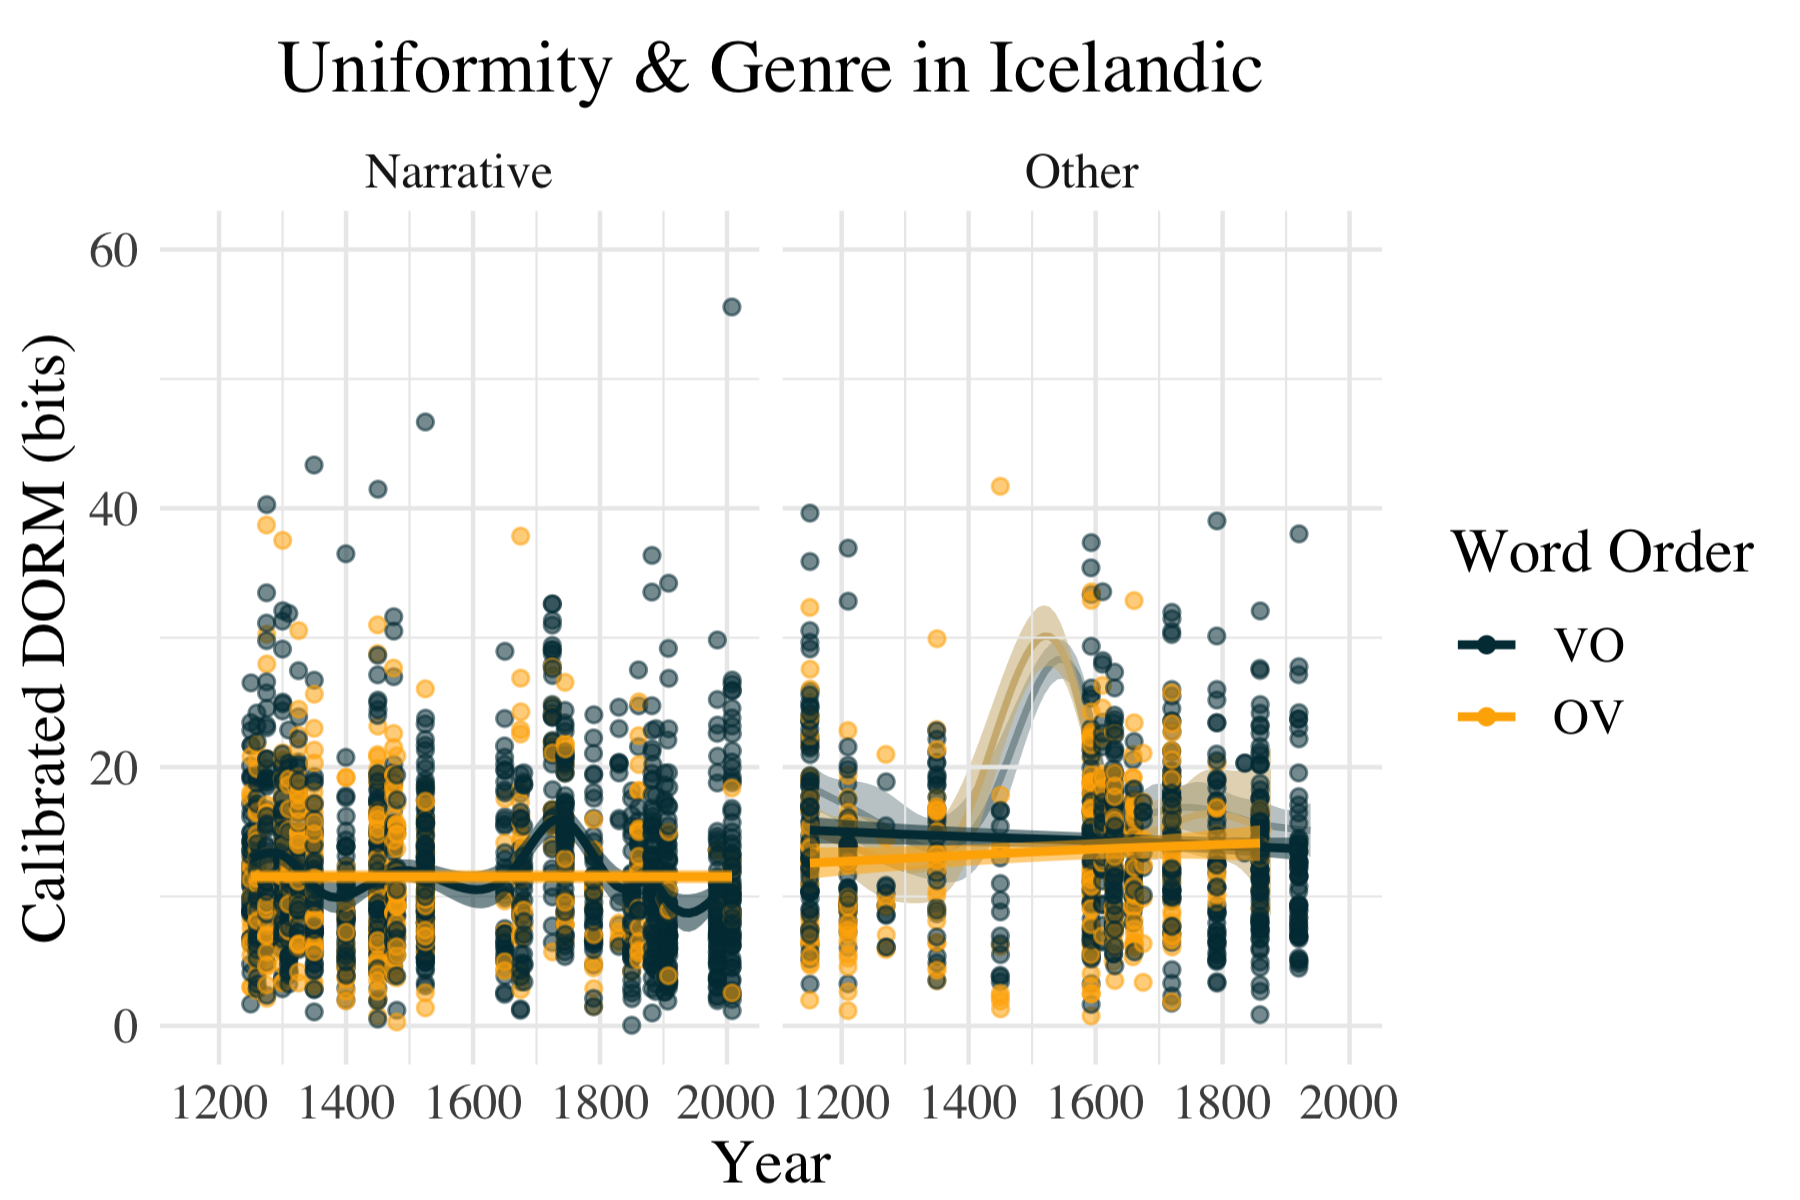
\includegraphics[scale = 0.2]{IcelandicGenreOutlierBehind.png}
%	\end{center}
	
\end{frame}


\begin{frame}{Conclusions} 
	
	
	\begin{itemize}
		\item It is exciting to be able to predict patterns of language change with this level of precision.\pause
		\item We \textbf{predicted and explained} a very subtle Constant Rate Effect on the OV-to-VO changes in both Icelandic and English, which is unexpected without an information theoretic approach.\pause
		\item The average uniformity of sentences is constant across the history of Icelandic.\pause
		\item Even while generations of speakers are participating in the OV-to-VO change, they use their syntactic resources to keep a target of information uniformity.\pause
		\item This complex unconscious planning could be a deep property of the linguistic system (and perhaps the memory system).
	\end{itemize}
	
\end{frame}


\begin{frame}{Future Directions} 
	
	
	\begin{itemize}
		\item \textbf{Replicate:} for historical English in lemmatised versions of the \textsl{Penn Parsed Historical Corpora}, and hopefully \textsl{York Corpus of Old English Prose} \citep{ycoe}\pause
		\item \textbf{Collaboration with Neuroscience:} Information uniformity, episodic memory, and ageing (Wallenberg, Smulders, Cuskley \& Read, \textsl{TBS to Scientific Reports})\pause
	\item \textbf{Public Engagement / Impact:} Centre for Life, National Centre for the Written Word\pause
		\item \textbf{Crazy idea}: language and ``ruin''\\ (collaboration with York Actuarial Science?)
	\end{itemize}
	
\end{frame}

\begin{frame}{Acknowledgements}
	\begin{center}
		
		Thanks to Rachael Bailes, Christine Cuskley, Tony Kroch, and colleagues at the CBE.\\This research was funded by ESRC grant ES/T005955/1.
		\url{https://github.com/joelcw/constantentropy}\\
		\url{https://github.com/joelcw/iceBits}\\\vspace{3mm}
		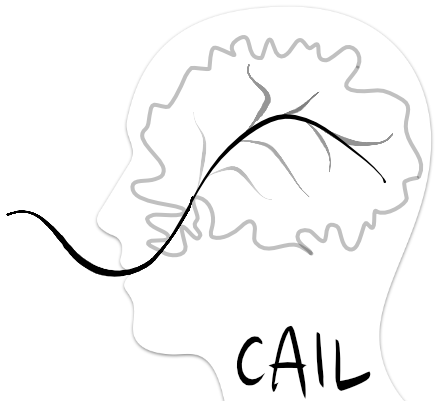
\includegraphics[scale = 0.2]{caillogo.png}
		
\includegraphics[scale = 0.4]{CBElogo.jpg}
	\end{center}
\end{frame}





\begin{frame}[allowframebreaks]
\frametitle{References}
\bibliographystyle{linquiry2}
\bibliography{joelrefs}
\end{frame}


\begin{frame}{Crash course} 
	\begin{itemize}
		\item The amount of information in a fair coin toss is 1 bit.
		\item The amount of information in an unfair coin toss with $$p = \frac{1}{3}, \frac{2}{3}$$ is less, even though less probable events have higher information content.
	\end{itemize}
	\begin{center}
		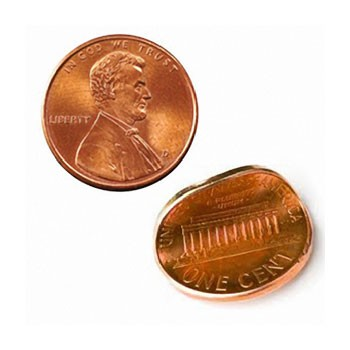
\includegraphics[scale=0.4]{bentcoin.jpg}
	\end{center}
\end{frame}

\begin{frame}{Statistics: OV-to-VO in English} 
	
	\begin{center}
		\texttt{OV $\sim$ Clause + zYear + SbjType + ObjType + SbjType*ObjType*zYear}\\\vspace{5mm}

\begin{tabular}{c c c}
\textbf{Term} & \textbf{$\beta$} & \textbf{p-value} \\ \hline
pronSbj:pronObj & -0.66 & 0.015\\
nomSbj:nomObj & -0.67 & 0.01 \\

	
\end{tabular}\\\vspace{5mm}

	Slope estimates not significantly non-zero for interaction with Text Date, $ 0.221 \leq p \leq 0.884$ depending on the argument combinations.
\end{center}

\end{frame}


\begin{frame}{Statistics: OV-to-VO in Icelandic} 
	
	\begin{center}
		\texttt{OV $\sim$ Clause + zYear + SbjType + ObjType + SbjType*ObjType*zYear}\\\vspace{5mm}

	\begin{tabular}{c c c}
		\textbf{Term} & \textbf{$\beta$} & \textbf{p-value} \\ \hline
		pronSbj:pronObj & -0.271 & 0.085\\
		nomSbj:nomObj & -0.271 & 0.085 \\
		nomSbj:quantObj & -0.554 & $9.36 \times 10^{-3}$
		
	\end{tabular}\\\vspace{5mm}

		Slope estimates not significantly non-zero for interaction with Text Date, $ 0.221 \leq p \leq 0.884$ depending on the argument combinations.
	\end{center}
	
\end{frame}

\begin{frame}{Statistics: OV and VO variation in historical Icelandic} 
	
	\begin{center}
		\texttt{SentDormUido $\sim$ (1 | TextId) + Year + OV + Clause + SimpleGenre +  ObjType + \\ SbjType + SbjType * ObjType * OV}\\\vspace{5mm}
	
	\begin{tabular}{c c c}
		\textbf{Term} & \textbf{$\beta$} & \textbf{p-value} \\ \hline
		pronSbj:pronObj:OV & 2.66 & 0.014\\
		nomSbj:nomObj:OV  & 2.66 & 0.014\\
		pronSbj:nomObj:OV  & -2.66 & 0.014\\
		nomSbj:pronObj:OV  & -2.66 & 0.014\\
	
		
	\end{tabular}\\\vspace{5mm}

		Effect of Text Date on calibrated DORM not significantly different from zero: \\$0.524 \leq p \leq 0.579$
	\end{center}
	
\end{frame}


\begin{frame}{``DORM'': Deviation of the Rolling Mean} 
	
	\begin{center}
		\begin{tabular}{c c c c c c}
			en & eg & skal & sjá & yður & aftur \\
			6.79 & 6.15 & 10.1 & 9.25 & 6.15 & 10.4\\
		\end{tabular}
	\end{center}
\end{frame}

\begin{frame}{``DORM'': Deviation of the Rolling Mean} 
	
	\begin{center}
		\begin{tabular}{c c c c c c}
			en & eg & skal & sjá & yður & aftur \\
			\textbf{6.79} & \textbf{6.15} & 10.1 & 9.25 & 6.15 & 10.4\\
			6.47 & & & & & 
		\end{tabular}
	\end{center}
	
\end{frame}

\begin{frame}{``DORM'': Deviation of the Rolling Mean} 
	
	\begin{center}
		\begin{tabular}{c c c c c c}
			en & eg & skal & sjá & yður & aftur \\
			6.79 & \textbf{6.15} & \textbf{10.1} & 9.25 & 6.15 & 10.4\\
			6.47 & 8.12 & & & & 
		\end{tabular}
	\end{center}
	
\end{frame}

\begin{frame}{``DORM'': Deviation of the Rolling Mean} 
	
	\begin{center}
		\begin{tabular}{c c c c c c}
			en & eg & skal & sjá & yður & aftur \\
			6.79 & 6.15 & \textbf{10.1} & \textbf{9.25} & 6.15 & 10.4\\
			6.47 & 8.12 & 9.67 & & & 
		\end{tabular}
	\end{center}
	
\end{frame}

\begin{frame}{``DORM'': Deviation of the Rolling Mean} 
	
	\begin{center}
		\begin{tabular}{c c c c c c}
			en & eg & skal & sjá & yður & aftur \\
			6.79 & 6.15 & 10.1 & \textbf{9.25} & \textbf{6.15} & 10.4\\
			6.47 & 8.12 & 9.67 & 7.70 & & 
		\end{tabular}
	\end{center}
	
\end{frame}

\begin{frame}{``DORM'': Deviation of the Rolling Mean} 
	
	\begin{center}
		\begin{tabular}{c c c c c c}
			en & eg & skal & sjá & yður & aftur \\
			6.79 & 6.15 & 10.1 & 9.25 & \textbf{6.15} & \textbf{10.4}\\
			6.47 & 8.12 & 9.67 & 7.70 & 8.29 & \\
		\end{tabular}
	\end{center}
	
\end{frame}

\begin{frame}{``DORM'': Deviation of the Rolling Mean} 
	
	\begin{center}
		\begin{tabular}{c c c c c c}
			en & eg & skal & sjá & yður & aftur \\
			6.79 & 6.15 & 10.1 & 9.25 & \textbf{6.15} & \textbf{10.4}\\
			6.47 & 8.12 & 9.67 & 7.70 & 8.29 & \\
		\end{tabular} \\\vspace*{5mm}
		Sample variance of rolling means = 1.33 bits\\
		(plus a further calibration for length and lexical idiosyncracy)\\\vspace*{3mm}
		\textbf{low DORM} $\rightarrow$ \textbf{more uniform}\\
		\textbf{high DORM} $\rightarrow$ \textbf{more lopsided}\\\vspace{4mm}\pause
		\textbf{Hypothesis_1:} When Sbj and Obj are same type, OV results in higher DORM.\\
		\textbf{Hypothesis_2:} When Sbj and Obj are different types, OV results in lower DORM.\\
		\textbf{Hypothesis_3:} These effects are orthogonal to the change (a CRE).\\
	\end{center}
	
\end{frame}




\end{document}